\documentclass[../main.tex]{subfiles}

\begin{document}
	\section{Pressure}
	\begin{preamb}
		These preambles are feeling more dreadful to write because pressure is building up.
	\end{preamb}

	\subsection{Pressure}
		\pdef{Pressure}{Pressure is defined as the amount of force per unit area. It is given as \[p = \frac{F}{A}\] The SI unit of pressure is the pascal [\si{\pascal}].}
		
	\subsection{Pressure of Fluids}
	\peqn{Pressure due to a Fluid Column}{Fluids of a density \(\rho\) can exert pressure \(p\) at a height \(h\) equal to}{p = \rho g h}
	\peqn{Transfer of Pressure}{Pressure is constant in an incompressible liquid,}{\frac{F_1}{A_1} = \frac{F_2}{A_2}}
	\peqn{Work Done}{Energy is conserved by the first law of thermodynamics (which is useful to keep in mind when solving hydraulic press problems):}{F_1 d_1 = F_2 d_2}

	\subsection{Atmospheric Pressure}
	\peqn{Atmospheric Pressure}{Atmospheric pressure at sea level is said to be \SI{1}{atm}. It is equal to \SI{101325}{\pascal}.}{p_0 = \SI{101325}{\pascal}=\SI{760}{\mmHg}}
	
	\peqn{Pressure Difference}{A manometer can be used to measure pressure differences. It measures a \(\Delta h\) which corresponds to a pressure difference of}{\Delta p = \rho g \Delta h}
	
	\begin{center}
		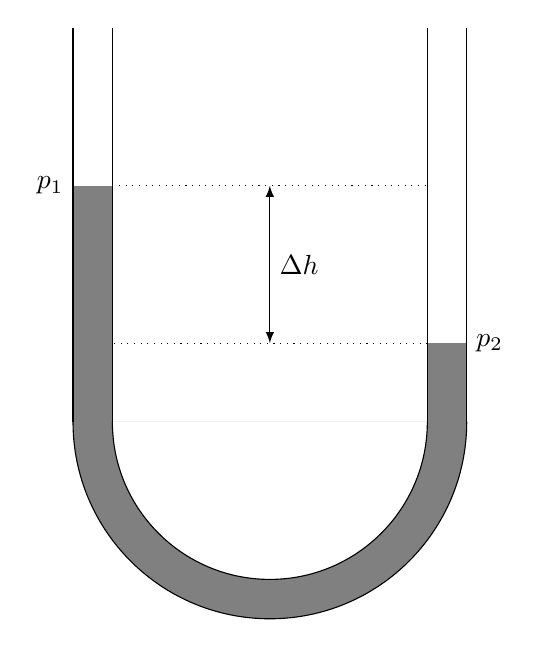
\begin{tikzpicture}
			\fill [gray] (0,0) --  (-4,0) arc (-180:0:2) -- (-4.5,0) -- (0.5,0) arc 	(0:-180:2.5);
			\fill [gray] (0.5,0) --  (0,0) -- (0,1) -- (0.5,1);
			\fill [gray] (-4,0) --  (-4.5,0) -- (-4.5,3) -- (-4,3);
			% \fill [white] (0,0) arc (0:-180:2) --  (-4,0);
			\draw (0,5) -- (0,0);
			\draw (0.5,5) -- (0.5,0);
			\draw (0,0) arc (0:-180:2);
			\draw (0.5,0) arc (0:-180:2.5);
			\draw (-4,5) -- (-4,0);
			\draw (-4.5,5) -- (-4.5,0);
			\path (-4.5,3) node[anchor=east] {\(p_1\)} -- (-4,3);
			\draw [dotted] (-4,3) -- (0,3);
			\path (0,1) -- (0.5,1) node[anchor=west] {\(p_2\)}; 
			\draw [dotted] (0,1) -- (-4,1);
			\draw [latex-latex] (-2,3) -- (-2,1) node[pos=0.5, anchor=west]{\(\Delta h \)};
		\end{tikzpicture}
		\[\Delta p = \left| p_2 - p_1 \right| = \rho g \Delta h\]
	\end{center}
	
\end{document}